\documentclass[a4paper,USenglish,numberwithinsect]{lipics}

\usepackage{graphicx}
\graphicspath{{figs/}}
\usepackage{latexsym}
\usepackage{url}
\usepackage{amssymb}
\usepackage{amsmath}
%\usepackage{amsthm}
\usepackage{amsfonts}
\usepackage{ifthen}
\usepackage{clrscode3e}
\usepackage{fancybox}
\usepackage{cite} % sort references within the same \cite command
\usepackage{enumerate} % fancy options for enumerate environment
\usepackage{microtype} % better line breaks and fewer overfull hboxes
\usepackage{varwidth}

\usepackage{todonotes}


%-- -- -- line numbers -- -- --
\usepackage[mathlines]{lineno}
\linenumbers
%-- -- -- line numbers -- -- --

%\usepackage{fullpage}

%\newtheorem{theorem}{Theorem}
%\newtheorem{corollary}[theorem]{Corollary}
%\newtheorem{lemma}[theorem]{Lemma}
%\newtheorem{problem}[theorem]{Problem}
%\newtheorem{proposition}[theorem]{Proposition}
%\newtheorem{conjecture}[theorem]{Conjecture}

\newcommand{\RR}{\ensuremath{\mathbb R}}  % real numbers
\newcommand{\ZZ}{\ensuremath{\mathbb Z}}  % integer numbers
\newcommand{\NN}{\ensuremath{\mathbb N}}  % natural numbers
\newcommand{\LL}{\ensuremath{\mathbb L}}  % 
\newcommand{\F}{\ensuremath{\mathcal{F}}}  
\newcommand{\D}{\ensuremath{\mathcal{D}}}  
\newcommand{\T}{\ensuremath{\mathcal{T}}}  
\newcommand{\GG}{\ensuremath{G_{\le 1}}}

\def\curve{\gamma}
\def\length{\mathit{len}}
\def\dist{\mathit{dist}}
\def\best{\mathit{best}}
\newcommand{\cycle}{\mathit{cycle}}
\newcommand{\walk}{\mathit{walk}}
\newcommand\CR{\mbox{\tt cr}_2}		  % crossing number

\def\DEF#1{\textbf{\emph{#1}}}
 
\let\leq\leqslant
\let\geq\geqslant
\let\le\leqslant
\let\ge\geqslant

\newcommand{\out}[1]{}

\def\myparagraph#1{\medskip\noindent\textbf{#1.}}


%%%%%%%%%%%%%%%%%%%%%%%%%%%%%%%%%%%%%%%%%%%%%%%%%%%%%%%%%%%%%%%%%%%%%%%%%%%%%%%%%%%%%%%%%%%%%%%%%%%%%%%%%%%%%%%%%%%%%%
\title{Two Optimization Problems for Unit Disks}
\titlerunning{Two Optimization Problems for Unit Disks}


\author[1]{Sergio~Cabello\footnote{Supported by the Slovenian Research Agency, program P1-0297 and project L7-5459.}}
\author[2]{Lazar~Milinkovi\'c}
\authorrunning{Sergio Cabello and Lazar~Milinkovi\'c}

\affil[1]{FMF, University of Ljubljana, and 
	Institute of Mathematics, Physics and Mechanics, Slovenia}
\affil[2]{FMF and FRI, University of Ljubljana, Slovenia}

%------------------------------ Text -------------------------------------

\begin{document}
\maketitle

\begin{abstract}
	To be done
\end{abstract}

%%%%%%%%%%%%%%%%%%%%%%%%%%%%%%%%%%%%%%%%%%%%%%%%%%%%%%%%%%%%%%%%%%%%%%%%%%%%%%%%%%%%%%%%%%%%%%%%%%%%%%%%%%%%%%%%%%%%%%
\section{Introduction}

In this paper we consider two geometric optimization problems in the plane
where unit disks play a prominent role. For both problems 
we discuss efficient algorithms to solve them, provide an implementation
of these algorithms, and present experimental results on the implementation.

The first problem we consider is computing a \emph{shortest-path tree} 
in the (unweighted) intersection graph of unit disks. 
The input to the problem is a set $\D$ of $n$ disks of the same size, 
each disk represented by its center.
The corresponding unit disk (intersection) graph has a vertex for each disk,
and an edge connecting two disks $D$ and $D'$ of $\D$ whenever $D$ and $D'$ intersect.
An alternative, more convenient point of view, is to take as vertex set the set of
centers of the disks, denoted by $P$, and connecting two points $p$ and $q$ of $P$ 
whenever the Euclidean length $|pq|$ is at most the diameter of a disk. 
Given a root $r\in P$, the task is to compute a shortest-path tree from $r$ in this graph.

The second problem we consider is the \emph{minimum-separation problem}.
The input is a set $\D$ of $n$ unit disks in the plane and two points
$s$ and $t$ not covered by any disks of $\D$.
We say that $\D$ \emph{separates} $s$ and $t$ if each curve in the plane 
from $s$ to $t$ intersects some disk of $\D$.
The task is to find the minimum cardinality subset of $\D$
that separates $s$ and $t$. Formally, we want to solve
\begin{align*}
	\min ~~		& |\D'|\\
	 \mbox{s.t.}~~ & \D'\subset \D \text{ and $\D'$ separates $s$ and $t$}. 
\end{align*}

Unit disks are the most standard model used for wireless sensor networks; 
see for example~\cite{GG11,HS95,zg-wsn-04}. 
Often the model is referred as UDG.
This model provides an appropriate trade off between simplicity and accuracy. 
Other models are more accurate, as for example discussed in~\cite{KWZ03,LP10},
but obtaining efficient algorithm for them is much more difficult.

While unit disks give a simple model, exploiting the geometric features 
of the model is often challenging. 
Shortest paths in unit disk graphs are essential for routing and
are a basic subroutine for several other more complex tasks. 
A somehow unexpected application of shortest paths in unit-disk graphs
to boundary recognition is given in~\cite{WGM06}.
The minimum-separation problem and variants thereof have been considered 
in~\cite{CG16,gkv-ipud-11,pv-2013}. 
The problem is dual to the barrier-resilience problem considered in~\cite{BK09,KH07,KLA05,KLA07}.
It is not obvious that the minimum-separation problem can be solved optimally
in polynomial time, and the known algorithm for this uses as a subroutine 
shortest paths in unit disk graphs. 
Thus, both problems considered in this paper are related and it is worth to 
consider them together.


\myparagraph{Our contribution}
We are aware of two algorithms to compute shortest-path trees in unit disk graphs in
$O(n\log n)$ worst-case time: one by Cabello and Jej\v{c}i\v{c}~\cite{CJ15} and one Efrat, Itai and Katz~\cite{eik-01}. 
Here we report on an implementation of a modification of the algorithm in~\cite{CJ15},
and compare it against two obvious alternatives.
The only complex ingredient in the algorithm is computing the Delaunay triangulation,
but efficient libraries are available for this.
The algorithm of~\cite{eik-01} would be substantially harder to implement 
and it has worse constants hidden in the $O$-notation. 

As mentioned before, it is not obvious that the minimum-separation problem 
can be solved in polynomial time. 
A 2-approximation algorithm is given by Gibson, Kanade, and Varadarajan~\cite{gkv-ipud-11}. 
Cabello and Giannopoulos~\cite{CG16} provide an exact algorithm that takes $O(n^3)$ 
wosrt-case time and works for arbitrary shapes, not just disks. 
In this paper we improve this last algorithm to near-quadratic time for the 
special case of unit disks. 
The basic principle of the algorithm is the same, but several additional tools
from Computational Geometry have to be employed to reduce the worst-case running time. 
We implement a variant of the new, near-quadratic-time algorithm and report
on the experiments.


\myparagraph{Assumptions} 
We will assume that \emph{unit disk} means that it has radius $1/2$. 
Up to scaling the input data, this choice is irrelevant.
However, it is convenient for the exposition
because then the disks intersect whenever 
the distance between their centers is $1$. 
The implementation and the experiments also make this assumption.

Henceforth $P$ will be the set of centers of $\D$. 
All the computation will be concentrated on $P$. 
In particular, we assume that $P$ is known.
(For the shortest path problem, one could possibly consider weaker models based 
on adjacencies. )

We will work with the graph $\GG(P)$ with vertex set $P$ 
and an edge between two points $p,q\in P$ 
whenever their Euclidean distance $|pq|$ is at most $1$. 
In the notation we remove the dependency on $P$ and just use $G$ instead of $\GG(P)$.
For simplicity of the theoretical 
exposition we will sometimes assume that $G$ is connected.
It is trivial to adapt to the general case, for example
treating each connected component separately.
The implementation does not make this assumption.

In the minimum-separation problem we will use $s$ and $t$
for the points to separate, we will assume that
the segment $st$ is vertical, $t$ is below $s$, and $t$ is 
at the origin. The implementation also makes
this assumption. A simple rigid transformation can be applied to
the input to get to this setting.

\myparagraph{Organization of the paper} 
In Section~\ref{sec:algorithms} we discuss the theoretical
algorithms for both problems and their guarantees.
In Section~\ref{sec:implementation} we discuss the implementations 
and in Section~\ref{sec:experiments} we present our experimental results.

%%%%%%%%%%%%%%%%%%%%%%%%%%%%%%%%%%%%%%%%%%%%%%%%%%%%%%%%%%%%%%%%%%%%%%%%%%%%%%%%%%%%%%%%%%%%%%%%%%%%%%%%%%%%%%%%%%%%%%
\section{Description of algorithms}
\label{sec:algorithms}

%%%%%%%%%%%%%%%%%%%%%%%%%
\subsection{Shortest-path tree in unit-disk graphs}
\label{sec:algorithm-sptree}
We describe here the algorithm of Cabello and Jej\v{c}i\v{c}~\cite{CJ15} 
to compute a shortest path tree in $G$ from a given root point $r\in P$. 
As it is usually done for shortest path algorithms 
we use tables $\dist[\cdot]$ and $\pi[\cdot]$ indexed by the points of $P$ to record, 
for each point $p\in P$, the distance $d_{G}(s,p)$ and the ancestor of $p$ 
in a shortest $(s,p)$-path. 

The pseudocode of the algorithm, which we call \proc{UnweightedShortestPath},
 is in Figure~\ref{fig:BFS}. 
We explain the intuition, taken almost verbatim from~\cite{CJ15}.
We start by computing the Delaunay triangulation $DT(P)$ of $P$. 
We then proceed in rounds for increasing values of $i$, 
where at round $i$ we find the set $W_i$ of points at distance exactly $i$ in $G$ from the source $r$. We start with $W_0=\{ r\}$. 
At round $i$, we use $DT(P)$ to grow a neighbourhood around the points of $W_{i-1}$ 
that contains $W_{i}$. 
More precisely, we consider the points adjacent to $W_{i-1}$ in $DT(P)$ as candidate points for $W_{i}$. For each candidate point that is found to lie in $W_{i}$, we also take its adjacent vertices in $DT(P)$ as new candidates to be included in $W_{i}$. For checking whether a candidate point $p$ lies in $W_{i}$ we use a data structure to find a nearest neighbour of $p$ in $W_{i-1}$. If the distance from $p$ to its nearest neighbour $w$ in $W_{i-1}$ is
smaller than $1$, then the shortest path tree is extended by connecting $p$ to $w$.

\begin{figure}[htb]
\begin{center}
\ovalbox{~~~~
\begin{varwidth}{\linewidth}
\begin{codebox}
    \Procname{$\proc{UnweightedShortestPath}(P,r)$}
    \li build the Delaunay triangulation $DT(P)$
    \li \For$p\in P$ \Do
    	\li $\dist[p] \gets \infty$
    	\li $\pi[p] \gets \const{nil}$\End
    \li $\dist[r] \gets  0$
    \li $W_0 \gets \{ r\}$
    \li $i\gets1$
    \li \While $W_{i-1}\neq\emptyset$ \Do
    	\li build data structure for nearest neighbour queries in $W_{i-1}$
    	\li $Q \gets W_{i-1}$ \>\>\>\Comment candidate points
        \li $W_{i}\gets\emptyset$
    	\li \While $Q\neq\emptyset$\Do
    		\li $q$ an arbitrary point of $Q$
            \li remove $q$ from $Q$
            \li \For $qp$ edge in $DT(P)$ \Do
            	\li $w \gets$ nearest neighbour of $p$ in $W_{i-1}$
            	\li \If $\dist[p]=\infty$ and $|pw|\leq 1$ \Then
                	\li $\dist[p]\gets i$
                    \li $\pi[p]\gets w$
                    \li add $p$ to $Q$
                    \li add $p$ to $W_{i}$
                    \End
            	\End
            \End
        \li $i\gets i+1$
    \End
    \li \Return $\dist[\cdot]$ and $\pi[\cdot]$
    \\[-2mm]
\end{codebox}
\end{varwidth}
~~~~}\end{center}
\caption{Algorithm from~\cite{CJ15} to compute a shortest path tree in the unweighted case.}
\label{fig:BFS}
\end{figure}

Cabello and Jej\v{c}i\v{c}~\cite{CJ15} show that the algorithm correctly computes
the shortest-path tree from $r$. 
If for nearest neighbors we use a data structure that,
for $n$ points, has construction time $T_c(n)$ and query time $T_q(n)$, 
and the Delaunay triangulation is computed in $T_{DT}(n)$ time,
then the algorithm takes $O(T_{DT}(n)+ T_c(n)+ n T_q(n))$ time. 
Standards tools in Computational Geometry imply that 
$T_{DT}(n)=O(n\log n)$, $T_c(n)=O(nqlog n)$ and $T_q(n)=O(\log n)$.
This leads to the following.

\begin{theorem}[Cabello and Jej\v{c}i\v{c}~\cite{CJ15}]
  Let $P$ be a set of $n$ points in the plane and let $r$ be a point from $P$. 
  In time ${\mathcal O}(n \log n)$ we can compute a shortest path tree from $s$
  in the unweighted graph $\GG(P)$.
\end{theorem}

It is clear that, when computing the shortest path tree from several sources,
we only need to compute the Delaunay triangulation once.

%%%%%%%%%%%%%%%%%%%%%%%%%%%%%%%%%%%%%%%%%%%%%%%%%%%%%%%%%%%%%%%%%%%%%%%%%%%%%%%%%%%%%%%%%%%%%%%%%%%%%%%%%%%%%%%%%%%%%%%%%%%%%
\subsection{Minimum separation with unit-disk}
\label{sec:algorithm-separation}

\subsubsection{Generic algorithm}
Cabello and Giannopouolos~\cite{CG16} present an algorithm
for the minimum separation problem that in the worst-case runs in cubic-time.
The algorithm has one feature that is both an advantage and a disadvantage: 
it works for any reasonable shapes, like segments or ellipses, and not just unit disks.
This means that it is very generic, which is good,
but it cannot exploit any properties of disks or unit disks.

The algorithm can be slightly simplified for disks, as we explain below. 
Let us first introduce some notation.
Each walk $W$ in the graph $G(P)$ defines a planar curve
in the obvious way: we connect the points of $P$ 
with segments in the order given by $W$. 
We will relax the notation slightly and denote also by $W$ the curve itself.
For any spanning tree $T$ of $G(P)$ and any edge $e\in E(G(P))\setminus E(T)$, 
let $\cycle(T,e))$ be the unique cycle in $T+e$.
Finally, for any walk in $G(P)$, let $\CR (st,W)$ be the 
modulo $2$ value of the number of crossings between the segment $st$ 
and (the curve defined by) $W$.

The following property is implicit in~\cite{CG16} and explicit in~\cite{CK15}:
\begin{quote}
	Let $T$ be any spanning tree of $G(P)$.
	The set of unit disks with centers in $P$ separate $s$ and $t$ if and only
	if there exists some edge $e\in E(G(P))\setminus E(T)$ 
	such that $\CR (st, \cycle(T,e))=1$.
\end{quote}

A consequence of this is that a minimum separation amounts to find a shortest
cycle $W$ in $G(P)$ such that $W$ crosses $st$ an odd number of times.
Moreover, one can show that we can restrict our search to the family 
of generating cycles. Indeed, for each root $r$ let us fix a 
shortest-path tree $T_r$ from $r$ in $G(P)$.
Then, we can restrict our search to
\[
	\{ \cycle(T_r,e)\mid r\in P,~ e\in E(G(P))\setminus E(T_r)\}.
\]
This follows from the co-called 3-path condition; 
see~\cite{CG16} for the details.

The values $\CR (st, \cycle(T_r,e))$ can be computed in amortized constant time
with a bit of bookkeeping. Consider a fixed $r$.
For each point $p\in P$ we store $N[p]$ as the parity of the number of crossings
of the path in $T_r$ from $r$ to $p$. When $p$ is not the root,
the value $N[p]$ can be computed from the value of its parent $\pi[p]$ in $T_r$
using that $N[p]=N[\pi[p]]+\CR(st,p\pi[p])$.
For each edge $pq\in E(G)$ we
then have $\CR (st, \cycle(T_r,pq))= N[p]+N[q]+\CR(st,pq)$ because
the crossings in the common part, from $r$ to the lowest common ancestor of $p$ and $q$,
cancel out modulo $2$.
The final resulting algorithm, denoted as \proc{GenericMinimumSeparation},
is given in Figure~\ref{fig:generic}.



\begin{figure}[htb]
\begin{center}
\ovalbox{~~~~
\begin{varwidth}{\linewidth}
\begin{codebox}
    \Procname{$\proc{GenericMinimumSeparation}(P,s,t)$}
    \li $\best \gets \infty$ // length of the best separation so far
    \li \For $s\in P$ \Do
    	\li $(\dist[~],\pi[~])\gets$ shortest path tree from $r$ in $G(P)$
		\\ \> \Comment Compute $N[~]$
    	\li $N[r]=0$
    	\li \For $p\in P\setminus \{r\}$ in non-decreasing values of $\dist[p]$ \Do
			\li $q\gets \pi[p]$
			\li $N[p]= N[q]+ \CR(st,pq) \pmod 2$
			\End
    	\li \For $pq\in E(G(P))$\Do
			\li \If $N[p]+N[q]+ \CR(pq,st) \pmod 2 =1$ \Then
				\li $\best \gets \min \{ \best, \dist[p]+\dist[q]+1$ 
				\End
			\End
		\End
    \li \Return $\best$
    \\[-2mm]
\end{codebox}
\end{varwidth}
~~~~}\end{center}
\caption{Adaptation of the generic algorithm to compute the minimum separation for unit disks.}
\label{fig:generic}
\end{figure}


\todo{Questions for the algorithm. Is this the algorithm that is implemented? 
Does it check wether $pq\in E(T_r)$? Do we compute $N(p)$ with the tree or later?}


Without loss of generality, in our theoretical discussion we will assume
that $z=(0,0)$ and $z'=(0,s)$. Therefore, $zz'$ is a segment, henceforth denoted by $\sigma$,
contained in the $y$-axis.

\subsubsection{Specialization for unit disks}




%%%%%%%%%%%%%%%%%%%%%%%%%%%%%%%%%%%%%%%%%%%%%%%%%%%%%%%%%%%%%%%%%%%%%%%%%%%%%%%%%%%%%%%%%%%%%%%%%%%%%%%%%%%%%%%%%%%%%%
\section{Implementation}
\label{sec:implementation}

%%%%%%%%%%%%%%%%%%%%%%%%%
\subsection{Shortest-path tree in unit-disk graphs}
\label{sec:implementation-sptree}

\myparagraph{Alternative constructions} 
Let us mention two obvious alternatives that we use in our comparison.

The first alternative is to build the graph $G=\GG(P)$ explicitly. 
Thus, for each pair of points $p,q$ we check whether their distance is
at most once and add an edge to a graph data structure.
We can then use breadth-first-search (BFS) from the given root $r$.
The preprocessing is quadratic, and the time spent to compute
a shortest-path tree depends on the density of the graph $G$.

The second option we consider is to use a unit-length grid. 
Two points $(x,y)$ and $(x',y')$ are in the same grid cell
if and only if 
$(\lfloor x\rfloor ,\lfloor y\rfloor)=(\lfloor x'\rfloor ,\lfloor y'\rfloor)$.
We store all the points of a grid cell $c$ in a list $\ell(c)$.
The non-empty lists $\ell(c)$ are stored in a dictionary,
where the bottom-left corner of the cell is used as key.
We can then run some sort of BFS using this data. When processing
a point $p$ in a cell $c$, we have to treat all the points 
in $c$ and its adjacent cells as candidate points. 
The preprocessing is linear, and the time spent to compute
a shortest-path tree depends on the density of the graph $G$.
The number of candidates that are checked is proportional to the
number of edges of the graph.
\todo{Are perhaps points deleted from the list once they are assigned a level?}


%%%%%%%%%%%%%%%%%%%%%%%%%
\subsection{Minimum separation with unit-disk}
\label{sec:implementation-separation}



%%%%%%%%%%%%%%%%%%%%%%%%%%%%%%%%%%%%%%%%%%%%%%%%%%%%%%%%%%%%%%%%%%%%%%%%%%%%%%%%%%%%%%%%%%%%%%%%%%%%%%%%%%%%%%%%%%%%%%
\section{Experimental results}
\label{sec:experiments}

Data was generated uniformly at random in polygons...


\begin{figure}
	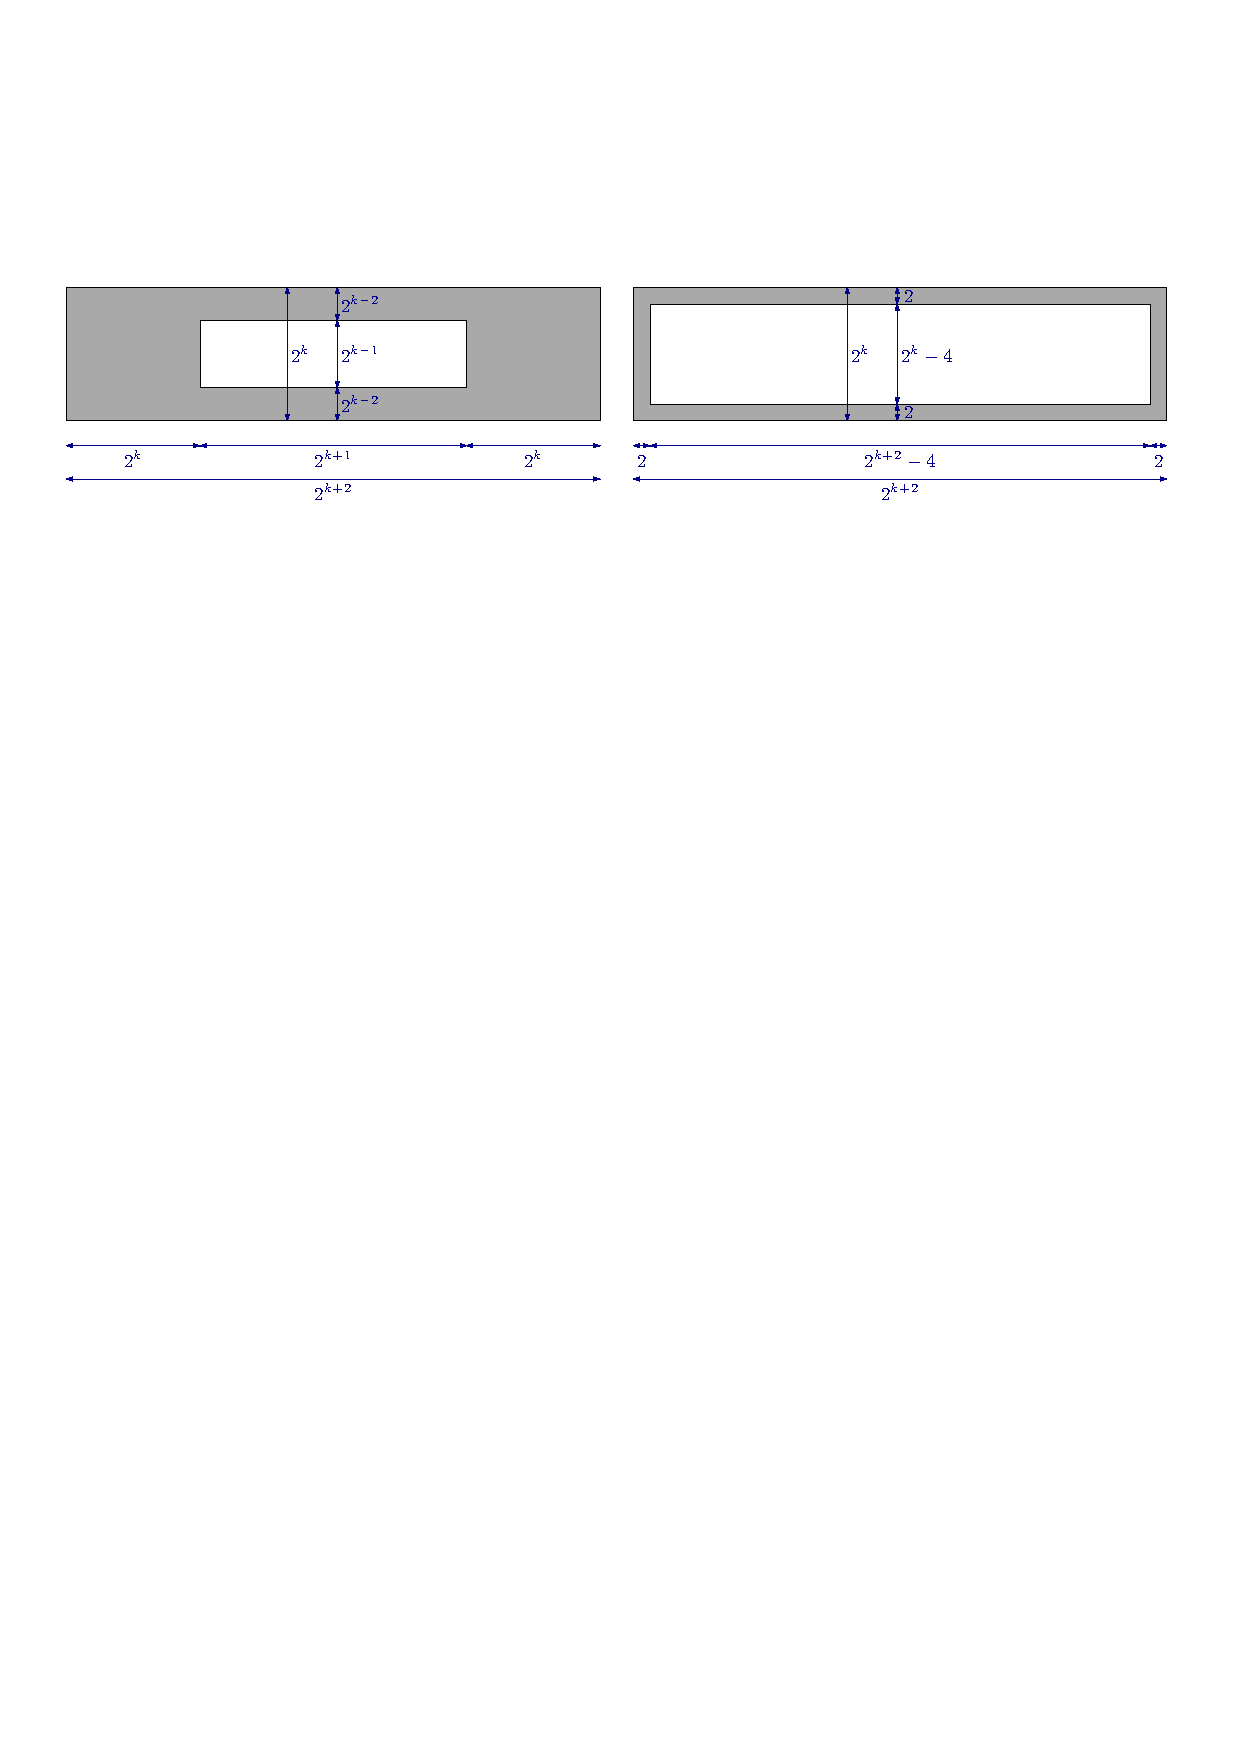
\includegraphics[width=\textwidth,page=1]{data_generation}
	\caption{Data generation with a small hole (left) and a large hole (right).}
	\label{fig:data_generation}
\end{figure}

\begin{figure}
	\includegraphics[width=\textwidth,page=2]{data_generation}
	\caption{Data generation with four small holes (right) and four large holes (right).}
	\label{fig:data_generation}
\end{figure}


%%%%%%%%%%%%%%%%%%%%%%%%%
\subsection{Shortest-path tree in unit-disk graphs}
\label{sec:experiments-sptree}

%%%%%%%%%%%%%%%%%%%%%%%%%
\subsection{Minimum separation with unit-disk}
\label{sec:experiments-separation}

%%%%%%%%%%%%%%%%%%%%%%%%%%%%%%%%%%%%%%%%%%%%%%%%%%%%%%%%%%%%%%%%%%%%%%%%%%%%%%%%%%%%%%%%%%%%%%%%%%%%%%%%%%%%%%%%%%%%%%
\section{Conclusions}
\label{sec:conclusions}





%%%%%%%%%%%%%%%%%%%%%%%%%%%%%%%%%%%%%%%%%%%%%%%%%%%%%%%%%%%%%%%%%%%%%%%%%%%%%%%%%%%%%%%%%%%%%%%%%
\bibliography{biblio}



\newpage
\begin{appendix}

%%%%%%%%%%%%%%%%%%%%%
\section{Building block}

The following ideas are probably folklore. See~\cite{aa}.

\begin{lemma}
\label{le:ds2}
	Let $P$ be a set of $n$ weighted points in the plane.
	In $O(n\log n)$ time we can construct a data structure that,
	for a query point $q$, it finds in time $O(\log^2 n)$ a point in
	\[	\arg\min \{ w_p \mid p\in P,~|pq|\le 1\}.
	\]
\end{lemma}
\begin{proof}
	We sort the points of $P$ by non-decreasing weight, build
	a balanced binary search tree $\T$ with $n$ leaves, and place
	the points of $P$ in the leaves of $\T$ such that the order
	arising from the search tree and the sorting of $P$ match.
	
	For every node $\nu$ of $\T$:
	\begin{itemize}
		\item Let $P(\nu)$ denote the set of points stored at the subtree rooted at $\nu$.
			We refer to $P(\nu)$ as a \emph{canonical subset}.
		\item Let $U(\nu)$ be the union of unit disks centered at the points of $P(\nu)$.
		\item We build a data structure to decide whether a given query point
			is contained in $U(\nu)$. A way to do this is to construct
			a point-location data structure for the Voronoi diagram of $P(\nu)$.
			Given a query point $q$, we find a closest neighbor from $P(\nu)$
			by locating a cell $c$ of the Voronoi diagram that contains $q$.
			We then check whether $q$ is at most at unit distance from the site defining $c$. 
			If the points of $P(\nu)$ are sorted (lexicographically),
			then the Voronoi diagram of $P(\nu)$ can be build in linear time~\ref{aaaa}
			The preprocessing time for node $\nu$ is $O(|P(\nu)|)$ and a
			query can be answered in $O(\log |P(\nu)|)= O(\log n)$ time.
	\end{itemize}
	
	This finishes the description of the construction of the data structure.
	Let us analyze the building time. We sort the points of $P$ 
	lexicographically at the root and for each node $\nu$ 
	we get the points $P(\nu)$ sorted from its parent.
	Since the canonical subsets at each level of the tree are disjoint,
	at each level of the tree we spend $O(n)$ time. 
	Since $\T$ is balanced, there are $O(\log n)$ levels and
	we spend in total $O(n\log n)$ time to build the data structure.
	
	Given a point $q$ we first check whether $q$ lies in $U(r)$ for the root $r$ of $\T$.
	If $q$ is not in $U(r)$, then no point of $P$ is close enough to $q$.
	Otherwise we set $\nu=r$ and proceed with a top-to-down search in the tree $\T$ 
	until we reach a leaf. 
	When $\nu$ is not a leaf, 
	let $\nu_\ell$ and $\nu_r$ be the left and right children of $\nu$, respectively. 
	If $q$ is in $U(\nu_\ell)$, we then proceed with the search in the subtree
	at $\nu_\ell$ by setting $\nu=\nu_\ell$,
	otherwise we proceed the search in the right subtree setting $\nu=\nu_r$.
	At each point of the search, we maintain the following invariant:
	\[	P(\nu) \cap \arg\min \{ w_p \mid p\in P,~|pq|\le 1\} ~\not=~ \emptyset.
	\].
	
	The search path in $\T$ has $O(\log n)$ nodes and, for each node in the path,
	spend $O(\log n)$ time to decide whether $q$ lies in $U(\nu)$. The total
	query time is thus $O(\log^2 n)$.	 
\end{proof}

Consider the following problem for two weighted point sets $A$ and $B$.
\begin{align*}
	\Phi(A,B) :=\min ~~		& w_a+w_b\\
	 \mbox{s.t.}~~ & a \in A, b\in B\\
				&	|ab|\le 1. 
\end{align*}

\begin{lemma}
\label{le:within}
	Let $A$ and $B$ be sets of at most $n$ weighted points in the plane.
	In $O(n\log^2 n)$ time we can compute $\Phi(A,B)$.
\end{lemma}
\begin{proof}
	We build the data structure of the previous Lemma for $B$.
	For each $a\in A$, we query the data structure to obtain
	\[	
		b^*(a) \in \arg\min \{ w_b \mid b\in B,~|ab|\le 1\}.
	\]
	Then we find the $a\in A$ minimizing the sum $w_a+w_{b^*(a)}$.	

	We need $O(n\log n)$ time to construct the data structure and 
	$O(\log^2 n)$ time per query. The result follows.
\end{proof}


Let $\sigma$ be a segment in the plane. 
Without loss of generality, we will assume that $s$ lies on
the $y$-axis with endpoints $(0,0)$ and $(0,s)$.
Let $A$ be a set of points with negative $x$-coordinates 
and let $B$ be a set of points with positive $x$-coordinates.
Each point $p$ of $A\cup B$ has a weight $w_p$.
We are interested in minimizing $w_a+w_b$ over all pairs $(a,b)\in A\times B$
whose segment $ab$ have length at most $1$ and intersects $s$.
Thus, we want to find
\begin{align*}
	\Phi_\sigma(A,B) :=\min ~~		& w_a+w_b\\
	 \mbox{s.t.}~~ & a\in A, b\in B\\
				&	|ab|\le 1\\
				&	\mbox{$ab$ intersects $\sigma$}. 
\end{align*}
For every point $a\in A$ we define the sets
\begin{align*}
	B(a)~&=~\{ b\in B\mid \text{$ab$ intersects $\sigma$}\},\\
	B_{\le 1}(a)~&=~ \{ b\in B\mid \text{$ab$ intersects $\sigma$ and $|ab|\le 1$}\} 
			~=~ \{ b\in B(a)\mid |ab|\le 1\}
\end{align*}
and the optimization problem
\begin{align*}
	\Phi_\sigma(a,B) = w_a + \min \{ w_b\mid b\in B_{\le 1}(a)\}.
\end{align*}
We thus have
\begin{align*}
	\Phi_\sigma(A,B) = \min_{a\in A} \Phi_\sigma(a,B).
\end{align*}

We first provide a data structure to obtain the sets $B(\cdot)$ compactly.
\begin{lemma}
\label{le:range}
	There is a family $\{ B_1,\dots, B_t\}$ of subsets of $B$
	and a data structure $\D (B)$ with the following properties
	\begin{itemize}
		\item $\sum_{i=1}^t |B_i| = O(n\log n)$;
		\item $\D (B)$ has size $O(n\log n)$ and can be constructed
			in $O(n\log n)$ time;
		\item for each point $a$ with negative $x$-coordinate, 
			there is a subset of indices 
			$I(a)\subset \{ 1,\dots,t\}$ such that $|I(a)|=O(\log^2 n)$ and
			$B(a)$ is the disjoint union of $\{ B_i \}_{i\in I(a)}$;
		\item for each query point $a$ with $a_x<0$, the data structure  $\D (B)$ returns $I(a)$
			in $O(\log^2 n)$ time.
	\end{itemize}
\end{lemma}
\begin{proof}
	It is convenient to use point-line duality. We use the precise duality
	described in BKOS Chapter XXX: the non-vertical line $\ell \equiv y=mx+c$
	is mapped to the point $\ell^*=(m,-c)$.
 
	Let $\LL$ be the set of non-vertical lines.
	Let $\sigma^*$ be the set of points dual to non-vertical lines that intersect $s$.
	Thus
	\[
		\sigma^* ~=~ \{ l^* \mid \ell\in \LL, \ell\cap \sigma\neq \emptyset\} 
	\]
	In the dual space, the set $\sigma^*$ is the horizontal slab 
	\[
		\sigma^* ~=~ \{ (m,-c)\in \RR^2\mid 0\le c\le s\}.
	\]
	
	For every point $b\in B$, let $L^* _b$ be the set of points dual
	to the lines through $b$ that intersect $\sigma$:
	\[
		L^*_b=\{ \ell^* \mid \ell\in \LL, b \in \ell, \text{ and } \sigma\cap \ell\not= \emptyset\}.
	\]
	In the dual space, $L^*_b$ is a segment with endpoints 
	$(\varphi_1(b),0)$ and $(\varphi_2(b),s)$, for some values $\varphi_1(b)$ and $\varphi_2(b)$
	that are easily computable.
	In particular, $L^*_b$ is contained in the slab $\sigma^*$ and has the endpoints on
	different boundaries of $\sigma^*$.
	Finally, define the mapping point $\varphi(b)=(\varphi_1(b),\varphi_2(b))$.
	Thus, $\varphi$ maps points to the right of the $y$-axis to points
	in the plane. Namely, $\varphi_1(b)$ is the slope of the line through $b$
	and $(0,0)$ while $\varphi_2(b)$ is the slope of the line through $b$ and $(0,s)$.

	Let $a$ be any point to the left of the $y$-axis and let $b\in B$.
	The segment $ab$ intersects $\sigma$ if and only if $L^*_a$ intersects $L^*_b$.
	Namely, an intersection of $L^*_a$ and $L^*_b$ is dual to the line
	through $a$ and $b$. The segments $L^*_a$ and $L^*_b$ intersect if
	and only if the order of their endpoints on boundaries of $\sigma^*$ are reversed.
	Thus we have the following property:
	\[
		ab \cap \sigma \neq \emptyset ~\Longleftrightarrow ~ 
		(\varphi_1(a)-\varphi_1(b)) \cdot (\varphi_2(a)- \varphi_2(b)) < 0.
	\]			
	Given a point $a$, the set of points $b\in B$ with the property
	that $ab$ intersects $\sigma$ corresponds to the points $b$ with $\varphi(b)$
	in 2 quadrants with apex $\varphi(a)$. 

	We can use a $2$-dimensional range tree to store the point set $\varphi(B)$,
	where each point $b\in B$ is identified with its image $\varphi(b)$. 
	For any query $a\in A$, the points $b\in B$ such that $ab$ intersects
	$\sigma$ are obtained by querying the 2-dimensional range tree for the points
	of $\varphi(B)$ contained in the two quadrants 
	\[
		\{(x,y)\mid  \varphi_1(a) > x \text{ and } \varphi_2(a) < y\} \cup
		\{(x,y)\mid  \varphi_1(a) < x \text{ and } \varphi_2(a) > y\}.
	\]
	The details are standard in computational geometry; see Chapter XXX of BKOS.
\end{proof}



\begin{lemma}
\label{le:accross}
	We can compute $\Phi_\sigma(A,B)$ in $O(n\log^4 n)$ time.
\end{lemma}
\begin{proof}
	We construct the sets $\{ B_1,\dots, B_t \}$ and the data structure $\D (B)$
	described in Lemma~\ref{le:range}. For each $B_j$, where $j=1,\dots , t$, 
	we build the data structure of Lemma~\ref{le:ds2}. 
	Since $\sum_{i=1}^t |B_i| = O(n\log n)$,
	we need
	\[
		\sum_{i=1}^t O(|B_i| \log |B_i|) ~=~ O(n\log^2 n)
	\]
	time for this.
	
	Consider a point $a\in A$. We query $\D (B)$ and obtain the 
	the set $I(a)$ of indices such that 
	\[
		B(a) ~=~ \bigcup_{i\in I(a)} B_i.
	\]
	Now, for each $i\in I(a)$, we query with $a$ the data structure associated 
	to $B_i$ to obtain
	\[	
		b_i^*(a) \in \arg\min \{ w_b \mid b\in B_i,~|ab|\le 1\}.
	\]
	We then have that
	\begin{align*}
		\min \{ w_b \mid b\in B_{\le 1}(a)\} ~=~ \min \{ w_{b_i^*(a)}\mid i\in I(a) \},
	\end{align*}
	so we can obtain $\Phi_\sigma(a,B)$ from the points $b_i^*(a)$, $i\in I(a)$. 
	
	For a point $a$, we need $O(\log^2 n)$ time to obtain $I(a)$,
	and then we need $O(\log^2 n)$ time for each index $i$ in $I(a)$. This means that
	we spend time $O(\log^4 n)$ for each point $a\in A$. 
\end{proof}


%%%%%%%%%%%%%%%%%%%%%%%%%%%%%%%%%%%%%%%%%%%%%%%%%%%%%%%%%%%%%%%%%%%%%%%%%%%%%%%%%%%%%%%%%%%
\section{Crossing a fixed segment}

We will drop in the notation the dependency on $P$ and just write $G$ instead of $G(P)$.
We will regard $G$ as an unweighted graph and denote by $d_G(r,p)$ the shortest-path
distance in $G$ between $r$ and $p$. 

For each point $r\in P$, let let $T_r$ be a shortest-path tree from $r$ in $G$.
If there are several possible candidates, we fix $T_r$.
We use $T_r[p]$ for the path in $T_r$ from $r$ to $p$.
Let $E_r$ be the set of edges of $G$ not appearing in $T_r$. 
Thus $E_r=E(G)\setminus E(T_r)$.

For each $r$ and $p$ from $P$, let $\curve(r,p)$ be the polygonal path
defined by $T_r[p]$.
For each $r\in P$ and each edge $pq\in E_r$, 
let $\curve(r,pq)$ be the polygonal closed path
obtained be concatenating $\curve(r,p)$, $pq$, and the reverse of $\curve(r,q)$.
We define $\length(r,pq)$ as the number of edges in $\curve(r,pq)$.
Thus we have $\length(r,pq) = d_G(r,p)+d_G(r,q)+1$.

Let $\sigma$ be a segment. For simplicity we assume that $\sigma$ does not
contain any point of $P$. For each polygonal path $\gamma$, let $X(\gamma,\sigma)$ be the
modulo two value of the number of crossings between $\gamma$ and $\sigma$.
For each $r,p\in P$ we define $N(r,p)=X(\curve(r,p),\sigma)$, and 
for each $r\in P$ and $pq\in E_r$ we define $N(r,pq)=X(\curve(r,pq),\sigma)$.

\begin{align*}
	\Psi_\sigma(P) := \min ~~& \length(r,pq)\\
	 \mbox{s.t.}~~ & r\in P\\
				&	pq\in E_r\\
				&	N(r,pq)=1. 
\end{align*}

The results of Cabello and Giannopoulos~\cite{aa} imply the following result.
(Should we provide a self-contained proof adapted to this scenario?)

\begin{theorem}
	Let $(r^*,p^*q^*)$ be an optimal solution to $\Psi_\sigma(P)$.
	Then the points in $T_{r^*}[p]\cup T_{r^*}[q]$ are an optimal solution
	to the separation problem.
\end{theorem}

To compute $\Psi_\sigma(P)$ we will iterate over the points $r$, so we define
\begin{align*}
	\Psi_\sigma(r,P) := \min ~~& d_G(r,p)+d_G(r,q) \\
	 \mbox{s.t.}~~ & pq\in E_r\\
				&	N(r,pq)=1. 
\end{align*}
We readily have
\[
	\Psi_\sigma(P) ~=~ 1+ \min_{r\in P} \Psi_\sigma(r,P)
\]

Let us fix some $r\in P$ and discuss how to solve $\Psi_\sigma(r,P)$. 
We compute a shortest path tree $T_r$ from $r$. Together with each
point $p\in P$ we store $d_G(r,p)$.

We compute the values $N(r,p)$, $p\in P$, with a simple bottom-up traversal of $T_r$.
We start setting $N_r[r]:=0$. For each point $p\in P$ whose parent in $T_r$ is $p'$,
we obtain $N_r[p]$ using that $N_r[p]=N_r[p']+ |\sigma\cap pp'| \pmod 2$.
This is, if $pp'$ crosses $\sigma$, then $N_r[p]=N_r[p']+1 \pmod 2$, otherwise
$N_r[p]=N_r[p']$.

Assume that $\sigma$ is a vertical segment with endpoints $(0,0)$ and $(0,s)$.

We split the search for the optimal edge $pq$ into cases: 
\begin{itemize}
	\item $pq$ has both endpoints on the same side of the $y$-axis and 
		connects points with $N(r,p)\neq N(r,p)$, or
	\item $pq$ has endpoints in both sides of the $y$-axis, $N(r,p)\neq N(r,p)$,
		and $pq$ does not intersect $\sigma$, or
	\item $pq$ has endpoints in both sides of the $y$-axis, $N(r,p)\neq N(r,p)$,
		and $pq$ intersects $\sigma$.
\end{itemize}


\begin{lemma}
\label{le:fixedr}
	We can compute $\Psi_\sigma(r,P)$ in $O(n\log^4 n)$ time.
\end{lemma}
\begin{proof}
	For $i\in \{0,1\}$, let $L_i$ be the subset of points of $P$ to the left of the $y$-axis
	with $N(r,p)=i\pmod 2$.
	For $i\in \{0,1\}$, let $R_i$ be the subset of points of $P$ to the right of the $y$-axis
	and $N(r,p)=i\pmod 2$.
	Clearly
	\[
		P~=~ L_0\cup L_1\cup R_0\cup R_1.
	\]
	
	Let $\sigma_+$ and $\sigma_-$ be the rays contained in the $y$-axis after deleting $\sigma$.
	Using $d_G(r,p)$ as the weight $w_p$ of point $p\in P$, 
	we then have
	\begin{align*}
		 \Psi_\sigma(r,P) ~=~ \min \{ &\Phi( L_0,L_1), \Phi( R_0,R_1),
										\Phi_{\sigma_+}( L_0,R_1), \Phi_{\sigma_+}( L_1,R_0),\\
										&\Phi_{\sigma_-}( L_0,R_1), \Phi_{\sigma_-}( L_1,R_0),
										\Phi_{\sigma}( L_0,R_0), \Phi_{\sigma}(L_1,R_1) \}.
	\end{align*}
	Each of these instances can be solved using Lemmas~\ref{le:within} and~\ref{le:accross} in
	$O(n\log^4 n)$ time.
\end{proof}


\begin{theorem}
	We can solve the minimum separation problem using $O(n^2\log^4 n)$ time.
\end{theorem}
\begin{proof}
	For each $r\in P$ we compute the shortest path tree $T_r$ from $r$ in $T$,
	the distances $d_G(r,p)$, $p\in P$, and the parities $N(r,p)$.
	We can then compute $\Psi_\sigma(r,P)$ using Lemma~\ref{le:fixedr}.
	
	Repeat for each $r\in P$.
	Time bound.
	
	Correctness.
	
\end{proof}


\end{appendix}
\end{document}